%\documentclass{acm_proc_article-sp}
\documentclass{sig-alternate}
%\usepackage{times}
\usepackage{verbatim}
\usepackage{bm}
\makeatletter
\newif\if@restonecol
\makeatother
\let\algorithm\relax
\let\endalgorithm\relax
\usepackage[lined,algonl,boxed]{algorithm2e}
\usepackage{multirow}
\usepackage{wasysym}
\usepackage{subfigure}
\usepackage{tabularx}

\newcommand{\reminder}[1]{\textbf{[** #1 **]}}  % to fix
\newcommand{\hide}[1]{} %hide
\newcommand{\vpara}[1]{\vspace{0.1in}\noindent\textbf{#1 }}
\newcommand{\para}[1]{\noindent\textbf{#1 }}
\newcommand{\secref}[1]{Section~\ref{#1}} %section reference
\newcommand{\Real}{\ensuremath{\mathbb{R}}}  % Real numbers
\newcommand{\figref}[1]{Figure~\ref{#1}} %section reference
\newcommand{\beq}[1]{\vspace{-0.01in}\begin{equation}#1\end{equation}\vspace{-0.01in}\normalsize}
\newcommand{\beal}[1]{\vspace{-0.01in}\begin{align}#1\end{align}\vspace{-0.01in}}
\newcommand{\beqq}[1]{\vspace{-0.01in}\begin{equation}#1\end{equation}\vspace{-0.01in}\normalsize}
%\newcommand{\eeq}[1]{\end{equation}\normalsize}
\newcommand{\besp}[1]{\begin{split}#1\end{split}}

\newdef{definition}{Definition}
\newdef{problem}{Problem}

\begin{document}

\conferenceinfo{WSDM'13,} {February 4--8, 2013, Rome, Italy.}
\CopyrightYear{2013}
\crdata{978-1-4503-1869-3/13/02}
\clubpenalty=10000
\widowpenalty = 10000

\title{Temporal Summarization of Knowledge Evolutionary Trend
%Learning to Infer Cross-Domain Collaborative Relationships}
}

\numberofauthors{3}
\hide{
\author{
\alignauthor Sen Wu\\
	\affaddr{Department of Computer Science}\\
	\affaddr{Tsinghua University}\\
	\affaddr{Beijing 100084, China}\\
	\email{ronaldosen@gmail.com}
\alignauthor Jimeng Sun\\
	\affaddr{IBM T. J. Watson Research Center}\\
	\affaddr{USA}\\
	\email{jimeng@us.ibm.com}
\alignauthor Jie Tang\\
	\affaddr{Department of Computer Science}\\
	\affaddr{Tsinghua University}\\
	\affaddr{Beijing 100084, China}\\
	\email{jietang@tsinghua.edu.cn}
}
}
\maketitle
\sloppy
%\input{abstract.tex}


\vspace{-0.1in}
% A category with only the three required fields
\category{J.4}{Social and Behavioral Sciences}{Miscellaneous}
\category{H.3.3}{Information Search and Retrieval}{Text Mining}
%\category{H.2.8}{Database Management}{Database Applications}
%\category{H.4.m}{Information Systems}{Miscellaneous}
\vspace{-0.06in}
\terms{Algorithms, Experimentation}
\vspace{-0.06in}
\keywords{Cross collaboration, Social network, Predictive model}


%\input{intro.tex}
%\section{Related Work}
\label{sec:related}

The technologies similar to 1)-3) have extensively been ex-plored in the area oftopic detection and tracking(TDT) (see [1]).Actually 1) and 2) are closely related to the subprob-lems in TDT called topic tracking andnew event detection, respectively.Here topic tracking is to classify texts into one of topics specified by a user, while new event detection, for-merly calledfirst story detection, is to identify texts that discuss a topic that has not already been reported in earlier texts.The latter problem is also related to work on topic-conditioned novelty detection by Yang et.al.[16]. In most of related TDT works, however, topic tracking or new event detection is conducted without identifying main topics or a topic structure, hence the tasks 1)-3) cannot be unified within a conventional TDT framework.Further topic time-line analysis has not been addressed in it.

Swan and Allen [12] addressed the issue of how to auto-matically overview timelines of a set of news stories. They used theχ $\chi^2$-method to identify at each time a burst of fea-ture terms that more frequently appear than at other times.

Similar issues are addressed in the visualization community [3]. However, all of the methods proposed there are not designed to perform in an on-line fashion.

Kleinberg [4] proposed a formal model of “bursts of activity” using an infinite-state automaton.This is closely related to topic emergence detection in our framework.A
burst has a somewhat different meaning from a topic in the sense that the former is a series of texts including a specific feature, while the latter is a cluster of categorized
texts.Hence topic structure identification and characterization cannot be dealt with in his model.Further note that Kleinberg’s model is not designed for real-time analysis but
for retrospective one.

Related to our statistical modeling of a topic structure, Liu et.al. [2] and Li and Yamanishi [6] also proposed meth-ods for topic analysis using a finite mixture model.Specifically, Liu et.al. considered the problem of selecting the optimal number of mixture components in the context of text clustering.In their approach a single model is selected as an optimal model under the assumption that the opti-mal model does not change over time. Meanwhile, in our approach, a sequence of optimal models is selected dynam-ically under the assumption that the optimal model may change over time.

Related to topic emergence detection, Matsunaga and Yamanishi [7] proposed a basic method of dynamic model se-lection, by which one can dynamically track the change of number of components in the mixture model.However, any of all of these technologies cannot straightforwardly be ap-plied to real-time topic analysis in which the dimension of data may increase as time goes by.

Related to topic structure identification, an on-line dis-counting learning algorithm for estimating parameters in a finite mixture model has been proposed by Yamanishi et. al.[14]. The main difference between our algorithm and theirs is that the former makes use of time-stamps in order to make the topic structure affected by a timeline of top-ics while the latter considers only the time-order of data ignoring their time-stamps.

The rest of this paper is organized as follows: Section 2 describes a basic model of topic structure.Section 3 gives a method for topic structure identification.Section 4 gives a method for topic emergence detection.Section 5 gives a method for topic characterization.Section 6 gives experimental results. Section 7 gives concluding remarks.
%\section{Problem Formulation}
\label{sec:problem}

In this section, we first present several necessary definitions and then define the tasks of temporal summarization.

\begin{definition}
\textbf{(Document)}:
We define a document $d$ as a sequence of $N_d$ terms, denoted as $\mathbf{w}_d$, where each term is chosen from a vocabulary of size $V$.
\end{definition}


\begin{definition}
\textbf{(Document Cluster)}: A document cluster, denoted as $C_q$, contains a set of documents relevant to the query $q$. The relevance can be considered as either syntax relevance (containing words in the query) or semantic relevance (containing relevant information of the query).
\end{definition}


\begin{definition}
\textbf{(Representative Term)}: Along the development of science, some concepts may dominate the research area in a specific period of time. For example, the concept deep learning is dominating the field of machine learning right now.
\end{definition}

\begin{definition}
\textbf{(Evolutionary Trend)}: An evolutionary trend $\mu$ of a document cluster $C$ is a set of term clusters over time, where terms can be assigned into different clusters at different time slides. Each document cluster is considered as a mixture of multiple topic models. The assumption of this model is that words in the document are sampled following word distributions corresponding to each topic, i.e., p(wjµ). Therefore, words with the highest probability in the distribution would suggest the semantics represented by the topic.
\end{definition}

The document cluster denotes the information source and the query denotes the information need. A document cluster is a sub set of the entire document collection. All documents in the cluster are related to the query. Thus, we can define the task of query-oriented temporal summarization as:

\begin{definition}
\textbf{(Query-based Temporal Summarization)}: Given a document collection $D$ and a query $q$ cluster $C$, the task of query-based temporal summarization is to identify the most representative terms and extract the evolutionary trend for the query, from the document cluster. Documents related to a query may talk about different perspectives of the query. For example, for the query "data mining", the topical aspects may include "classification", "clustering", and "association rule". Accordingly, we give definitions of the topic model and the query-oriented topic model of a document cluster.
\end{definition}


For the example of "data mining", suppose the query is about data mining application, we may only want to high-light topics related to applications of data mining algorithms
and treat the other topics in the second place. Table 1 summarizes the notations.
Based on these definitions, the major task of query-oriented summarization can be defined as follows: given a query and a document collection, the goal is to retrieve a
document cluster related to the query and summarize the document cluster from different topical aspects of the query. It is challenging to perform the task defined above.
First, existing topic models only consider the general topic distribution of multiple documents, but cannot capture the query information. It is challenging on how to incorporate the query information into the topic model and how to discriminate the different topics in the document cluster in a principled way. Second, it is unclear how to make use of the modeling results to calculate the score of each sentence and how to generate the final summarization result.

\section{Domain Knowledge}
\label{sec:approach}

The standard topic modeling techiques decomposing the observed data into latent topics according to a purely data-driven objective function. This means that topic models inherit some of the disadvantages of unsupervised learning. For example, there may be multiple candidate partitions of the dataset which capture different aspects of the underlying structure.

Purely unsuperivsed topic modeling discover topics which represent strong statistical patterns but do not always correspond to user expectations of semantically meaningful topics. 

Supervised LDA[Blei and McAuliffe, 2008] can be applied to labeled documents, augmenting each document $d$ with a label variable $y_d$, which either categorical or continuous. Each $y_d$ value is modeled by a Generalized Linear Model in the vector of mean topic counts $\bar{Z} = \frac{1}{N_d}\sum_{N_d}^{n=1}z_n$ for the document. This approach can therefore make label prediction by calculating the posterior topic assignments for a test document to obtain a $\bar{z}$ value. This model tends to produce topics that are able to "explain" the label value $y$ for the training set. In this way the label information indirectly influences the topic decomposion discovered by the model.

In dynamic topic models, the corpus is partitioned into disjoint time slices. Using logistic normal distributions, both the document-topic mixtures and topic-word multinomials evolve via multivariate Gaussian dynamics (i.e., at time step $s$ natural parameter $v_s$ is Gaussian distributed with mean $v_{s-1}$). Topics over time modeling timestamps as being genreated by the model itself. 

In standard LDA, topic-word multinomial distributions $\Phi_z = p(w|z)$ are drawn from a Dirichlet prior with hyperparameter $\beta$. To some extent, domain knowledge can be encoded into this Dirichlet prior by setting the values in the $\beta$ hyperparameter vector. The standard Dirichlet prior can be replaced with a more expressive Dirichlet Forest Prior.

The Dirichlet Tree distribution reparameterizes and generalized the standard Dirichlet distribution, while maintaining conjugacy to the multinomial. In the Dirichlet Tree, the leaf nodes correspond to the mulitnomial probabilities. The root node is assigned probability mass 1, which then "flows" to its children in proportion to a sample from Dirichlet distriution parametrized by the out-edge weights. Each internal node then distributes the probability mass it recives to its children in the same way.

The Dirichlet forest prior encodes both "Must-Link" and "Cannot-Link". It yeilds a mixture model of Dirichlet subtree within each connected component, each corresponds to a maximal clique. For each topic, one subtree is selected according to probability $$P(r) = |M_{rq}|, q = 1...Q^{(r)}.$$
Enssentially the selected subtree indexed by $q$ tends to redistribute nearly all probability mass to the words within $M_{rq}$. Since there is no mass left for other cliques, it is impossible for a word outside clique $M_{rq}$ to have a large probability. Therefore, no Cannot-Link will be violated.

LogicLDA allows the user to express domain knowledge in First-Order Logic. 
\begin{itemize}
\item \textbf{Constants} are symbols that represent an actual object in the problem domain.
\item \textbf{Variables} are symbols that can take on values from the set of constants.
\item \textbf{Predicates} are symbols that express relations, and evaluate to \emph{true} or \emph{false} for different arguments.
\item \textbf{Functions} are symbols that express mappings.
\item \textbf{Terms} are any expressions that refer to objects in the domain.
\item \textbf{Atoms} are predicates applied to terms.
\item \textbf{Formulas} are constructed from atoms using logical connectives $(\wedge,\vee,\neg,\Rightarrow)$.
\item \textbf{Clauses} are formulas consisting of a disjunction of literals.
\item \textbf{Ground} terms, atoms, or formulas contain no variables.
\end{itemize}

Markov Logic Networks are a class of graphical models operate over this type of logical domain. A "possible world" consists of a set of binary assignments for all possible ground predicates. A MLN then assigns probabilities to all possible worlds. 

\begin{itemize}
\item $Z(i,t)$ is true if the hidden topic $z_i = t$, and false otherwise.
\item $W(i,v)$ is true if word $w_i = v$, and false otherwise.
\item $D(i,j)$ is true if $d_i = j$, and false otherwise.
\end{itemize}

The model probability of LogicLDA can be interpreted as the product of the individual MLN and LDA contributions. Another perspective is that LogicLDA consists of an MLN augmented with continuous varibles $(\Theta, \Phi)$ and associated potential functions.

The goal of LogicLDA is to learn the most likely $\phi$ and $\theta$ in the model. As in standard LDA, the latent topic assignment $z$ cannot be marginalized out in practice due to their combinatorial nature. We instead aim to find the maximum a posteriori estimate of $z$, $\Theta$, $\Phi$ jointly. This can be formulated as maximizing the logarithm of the unnormalized probability.
\section{Summarization Framework}
\label{sec:algorithm}

The major motivation of our work is to find a concise and intuitive summarization of a given research topic. More concretely, we want to select a set of representative terms that best describe the hot spots and major achievements along the development of the research topic, meanwhile, capture the temporal evolutionary pattern within the research area. We formulated the problem as a graph partitioning task. At a high level, the proposed summarization framework consists of three stages.

\begin{itemize}
    \item {\bf Document retrieval.} First, given a research topic $q$ needs to be summarized, we find a documents collection $D = \{d_t\}^T$ that can represent the development of the research topic, where $d_t$ denote the documents at time $t$.
    
    \item {\bf Dynamic concept graph construction.}  
    Second, we extract knowledge concept terms mentioned in each document and construct a graph $G$, where each term $w_i$ at time slide $t$ is associated with a node $n_i^t$. We explicitly model the semantic relationship and evolving patterns with the graph by associating feature scores on the nodes and edges.
    
    \item {\bf Trend partitioning.} Third, we utilize a message passing algorithm on the constructed dynamic concept graph to select a set of terms based on their \emph{authority}, \emph{burstiness} and network structures, and further partition the graph into evolutionary trends.
\end{itemize}

\subsection{Document Retrieval}

To summarize a given research topic $t$ (i.e., user's query), we need to first map the topic to a set of documents. A straightforward idea is to use some traditional information retrieval technique to find the relevant documents. However, such an approach is not appropriate for the dynamic summarization task due to the following reasons. First, we want to summarize the development of the topic over time, if we use such an approach, we won't be able to trace how a knowledge concept evolve from and emerge into some other related concepts. Second, it has obvious bias that most retrieved documents will contain the queried words. Third, if a query contains a rare used term or a new term, it will face the problem of data sparseness. 

To overcome the disadvantages above, we use a community-base document retrieval method. We first find a core research community (a group of experts) related to the topic, and then aggregate all the members' research work as the document collection to summarize. Such an approach is very intuitive since these researchers are leading the development the research area. To avoid some authoritative experts' work dominated in the documents and introduce potential bias, we normalize each member's contribution averagely.

\subsection{Dynamic Concept Graph Construction}
After the initial retrieval of related document collection, we extract knowledge concepts mentioned in each documents. In this work, we simply use wikipedia titles as a vocabulary to extract terms. With the extracted terms of each document over time, we construct a dynamic concept graph $G=\{V,E_r,E_e\}$ to model the semantic relationship and evolutionary pattern between terms uniformly. For a term $w_i$, we create a node $n_i^t$ for each time slide $t$. There are two types of edges in the graph, $E_r$ are representative edges denotes how well-suited for a term to act as a representative of another term at a given time. $E_e$ are evolving edges connecting the same terms within two adjacent time slides indicating to what extent the meaning of the term has shifted.

\begin{center}
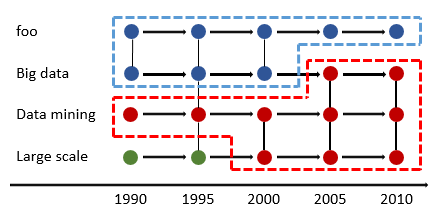
\includegraphics[width=0.80\linewidth]{figures/mutual.png}
\end{center}

\begin{itemize}

\item \textbf{Representativeness:} 
To capture the semantic relationship between terms, we connect terms co-occurred in the documents at the same time slide with representative edges. Formally, the weight of the directed edge $(n_i^t,n_j^t)$ is defined based on mutual information, indicates how appropriate it is to use term $w_i$ to represent $w_j$ at time $t$. We calculate mutual information between term $w_i$ and term $w_j$ at the given time slide $t$ as:
\begin{equation}
\begin{split}
I(n_i^t,n_j^t) & = p(w_i \in d_t, w_j \in d_t)log{\frac{p(w_i\in d_t, w_j \in d_t)}{p(w_i \in d_t)p(w_j \in d_t)}} \\
& + p(w_i \in d_t, w_j \notin d_t)log{\frac{p(w_i\in d_t, w_j \notin d_t)}{p(w_i \in d_t)p(w_j \notin d_t)}} \\
& + p(w_i \notin d_t, w_j \in d_t)log{\frac{p(w_i\notin d_t, w_j \in d_t)}{p(w_i \notin d_t)p(w_j \in d_t)}} \\
& + p(w_i \notin d_t, w_j \notin d_t)log{\frac{p(w_i\notin d_t, w_j \notin d_t)}{p(w_i \notin d_t)p(w_j \notin d_t)}}
\end{split}
\end{equation}

where $d_t$ denotes all the retrieved documents at time $t$. The representativeness of term $w_i$ to term $w_j$ at time $t$ is then defined as normalized mutual information $$s(n_i^t,n_j^t) = \frac{I(n_i^t,n_j^t)}{I(n_i^t,I_i^t)}$$


\item \textbf{Meaning shift:}
Nodes corresponding to the term $w_i$ within two adjacent time slides $-1t$ and $t$ are connected by an evolving edge $(n_i^{t-1},n_i^{t})$, indicates that the term is evolved from itself at the last time slide. The weight of the evolving edge indicates whether the meaning of the term is staying the same or shifted from time $t-1$ to $t$. Formally the weight is defined based on Jaccard coeffient.
$$s(n_i^{t-1},n_i^t) = \frac{|NB(n_i^{t-1}) \cap NB(n_i^t)|}{|NB(n_i^{t-1}) \cup NB(n_i^t)|}$$

\item \textbf{Burstiness:}
We model burstiness by assuming the arrival of terms as an unknown binomial distribution, and use $\chi^2$ tests to check for significant association between words and time periods. We calculate the contingency table as below and $\chi^2 = \frac{(ad-bc)^2n}{(a+b)(c+d)(a+c)(b+d)}$.
\begin{center}
\begin{tabularx}{0.5\linewidth}{ |X|X|X| }
  \hline
  - & $W$ & $\bar{W}$ \\
  \hline
  $t$  & a  & b  \\
  \hline
  $<t$  & c  & d  \\
  \hline
\end{tabularx}
\end{center}

We define burstiness of term $w_i$ at time $t$ as $b_i^t = \chi^2$ value.

\item \textbf{Authority:}
We simply defined the authority of a term at a given time by $u_i^t=df_t(w_i)/|d_t|$, where $df_t(w_i)$ indicates the document frequency of $w_i$ at time $t$, and $|d_t|$ is the number of documents at time $t$.
\end{itemize}




\subsection{Trend Partitioning}
In order to give a concise and intuitive summarization, we need to partition the dynamic concept graph into evolutionary trends, and select a set of representative terms best describe the development of the research topic. Here, we use a massage passing algorithm to perform the selection and partition. The method is analogous to affinity propagation(AP) algorithm proposed in Frey et al. and Tang et al, the difference is that our method is modified to fit the dynamic setting. The AP algorithm performs clustering by identifying exemplars. Essentially it solves the following optimization problem
$$c^* = argmin(-\sum S(i,c_i) )$$
where $C=(c_i)$ is the mapping between nodes and exemplars, $S(i,c_i)$ indicates the similarity between $i$ and its exemplar. $S(i,i)$ is the penalty for i to being exemplar of itself.

In the algorithm, we introduce three sets of variables $\{r_{ij}^t\}$, $\{a_{ij}^t\}$ and $\{e_i^{t-1,t}\}$. Where $r_{ij}^t$ indicates the how well-suited term $w_j$ is to serve as an exemplar of term $w_i$ (i.e. $w_j$ covers the meaning of $w_i$) at time slide $t$. $a_{ij}$ denotes the availabilities of term $w_j$ to serve as an exemplar of $w_i$ at time $t$. $\{e_i^{t-1,t}\}$ indicates the equivalence between the term $w_i$ at two adjacent time slides which captures to what extent the meaning of term $w_i$ has shifted from $t-1$ to $t$.
All the $r_{ij}^t$, $a_{ij}^t$ and $e_i^{t-1,t}$ are set to $0$ initially, their values are updated iteratively with following rules until convergence.
\beal{
r_{ij}^t = (1-\lambda)\rho_{ij}^t+\lambda r_{ij}^t\\
a_{ij}^t = (1-\lambda)\alpha_{ij}^t+\lambda a_{ij}^t
}
where $\lambda$ is a damping factor, $\rho_{ij}^t$ and $\alpha_{ij}^t$ are messages passing from $n_i^t$ to $n_j^t$. The massage passing rules are defined as follows:


\beal{
\rho_{ij}^t = s(n_i^t,n_j^t) - \max_{k\in NB(n_j^t)}\{s(n_i^t,n_k^t) + a_{ik}^t\}\\
\alpha_{ii}^t = \sum_{k\in NB(n_i^t)}\max\{0,r_{ij}^t\}\\
\alpha_{ij}^t = min\{0,r_{jj}^t + \sum_{k \in NB(n_j^t)}\max\{0,r_{ik}^t\}\}
}

\begin{algorithm}[t]
\label{alg:learning}
\caption{Message passing algorithm on dynamic concept graph.}
\small
% factor graph learning
%Learning step:
%\BlankLine
\SetLine \KwIn{dynamic concept graph $G=\{V,E_r,E_e\}$;}
\KwOut{a set of representative nodes $V_r$ and the par;}
%// Generate train data\;
%$G=\emptyset$\;
Initialize all ${r_{ij}^t}\leftarrow\mathbf{0}$\;
\Repeat{converge}{
    \ForEach{edge ($n_i^t$)}{
     //Initialization\;
    $L \leftarrow$ initialization list\;
    %$inventorction(L)$\;
    %$L \leftarrow RemoveUnlabelNodes(L)$\;

%\BlankLine
Factor graph $FG \leftarrow BuildFactorGraph(L)$\;

// Learn the parameter $\mathbf{\theta}$ for factor graph model\;
%$order \leftarrow BuildUpdateOrder(FG)$\;

\Repeat{(all messages $\mu$ do not change)}{
    \ForEach {$v_i \in order$} {
        Update the messages of $v_i$\ by Eqs.~\ref{eq:sp_v} and \ref{eq:sp_f};
    }
}
\ForEach{$\theta_i\in \mathbf{\theta}$} {
    Calculate gradient $\nabla_i$ according to Eq. \ref{eq:gradient}\;
    Update $\theta^{new} = \theta^{old} + \eta \cdot \nabla_i$\;
}
}
}
\normalsize
\end{algorithm}

where $NB(n_j^t)$ denotes the neighboring nodes of node $n_j^t$, $s(n_i^t,n_j^t)$ is $w_i$'s representativeness of $w_j$ at time $t$. $s(n_i^t,n_i^t)$ is set to $s(n_i^t,n_i^t) = \beta b_i^t + (1-\beta)u_i^t$ indicates that the nodes with high authority and burstiness are preferred to be choose as exemplars, where $\beta$ is a parameter controlling the trade-off between timeliness and importance. 




%\input{observation.tex}
%\input{exp.tex}
%\input{exp_new.tex}
%\section{Related Work}
\label{sec:related}

The technologies similar to 1)-3) have extensively been ex-plored in the area oftopic detection and tracking(TDT) (see [1]).Actually 1) and 2) are closely related to the subprob-lems in TDT called topic tracking andnew event detection, respectively.Here topic tracking is to classify texts into one of topics specified by a user, while new event detection, for-merly calledfirst story detection, is to identify texts that discuss a topic that has not already been reported in earlier texts.The latter problem is also related to work on topic-conditioned novelty detection by Yang et.al.[16]. In most of related TDT works, however, topic tracking or new event detection is conducted without identifying main topics or a topic structure, hence the tasks 1)-3) cannot be unified within a conventional TDT framework.Further topic time-line analysis has not been addressed in it.

Swan and Allen [12] addressed the issue of how to auto-matically overview timelines of a set of news stories. They used theχ $\chi^2$-method to identify at each time a burst of fea-ture terms that more frequently appear than at other times.

Similar issues are addressed in the visualization community [3]. However, all of the methods proposed there are not designed to perform in an on-line fashion.

Kleinberg [4] proposed a formal model of “bursts of activity” using an infinite-state automaton.This is closely related to topic emergence detection in our framework.A
burst has a somewhat different meaning from a topic in the sense that the former is a series of texts including a specific feature, while the latter is a cluster of categorized
texts.Hence topic structure identification and characterization cannot be dealt with in his model.Further note that Kleinberg’s model is not designed for real-time analysis but
for retrospective one.

Related to our statistical modeling of a topic structure, Liu et.al. [2] and Li and Yamanishi [6] also proposed meth-ods for topic analysis using a finite mixture model.Specifically, Liu et.al. considered the problem of selecting the optimal number of mixture components in the context of text clustering.In their approach a single model is selected as an optimal model under the assumption that the opti-mal model does not change over time. Meanwhile, in our approach, a sequence of optimal models is selected dynam-ically under the assumption that the optimal model may change over time.

Related to topic emergence detection, Matsunaga and Yamanishi [7] proposed a basic method of dynamic model se-lection, by which one can dynamically track the change of number of components in the mixture model.However, any of all of these technologies cannot straightforwardly be ap-plied to real-time topic analysis in which the dimension of data may increase as time goes by.

Related to topic structure identification, an on-line dis-counting learning algorithm for estimating parameters in a finite mixture model has been proposed by Yamanishi et. al.[14]. The main difference between our algorithm and theirs is that the former makes use of time-stamps in order to make the topic structure affected by a timeline of top-ics while the latter considers only the time-order of data ignoring their time-stamps.

The rest of this paper is organized as follows: Section 2 describes a basic model of topic structure.Section 3 gives a method for topic structure identification.Section 4 gives a method for topic emergence detection.Section 5 gives a method for topic characterization.Section 6 gives experimental results. Section 7 gives concluding remarks.
%\input{conclusion.tex}

%\small
\bibliographystyle{abbrv}
%\bibliography{references-full}
% sigproc.bib is the name of the Bibliography in this case
\begin{thebibliography}{10}


\end{thebibliography}

\normalsize

\end{document}
